% Options for packages loaded elsewhere
\PassOptionsToPackage{unicode}{hyperref}
\PassOptionsToPackage{hyphens}{url}
%
\documentclass[
]{article}
\usepackage{amsmath,amssymb}
\usepackage{iftex}
\ifPDFTeX
  \usepackage[T1]{fontenc}
  \usepackage[utf8]{inputenc}
  \usepackage{textcomp} % provide euro and other symbols
\else % if luatex or xetex
  \usepackage{unicode-math} % this also loads fontspec
  \defaultfontfeatures{Scale=MatchLowercase}
  \defaultfontfeatures[\rmfamily]{Ligatures=TeX,Scale=1}
\fi
\usepackage{lmodern}
\ifPDFTeX\else
  % xetex/luatex font selection
\fi
% Use upquote if available, for straight quotes in verbatim environments
\IfFileExists{upquote.sty}{\usepackage{upquote}}{}
\IfFileExists{microtype.sty}{% use microtype if available
  \usepackage[]{microtype}
  \UseMicrotypeSet[protrusion]{basicmath} % disable protrusion for tt fonts
}{}
\makeatletter
\@ifundefined{KOMAClassName}{% if non-KOMA class
  \IfFileExists{parskip.sty}{%
    \usepackage{parskip}
  }{% else
    \setlength{\parindent}{0pt}
    \setlength{\parskip}{6pt plus 2pt minus 1pt}}
}{% if KOMA class
  \KOMAoptions{parskip=half}}
\makeatother
\usepackage{xcolor}
\usepackage[margin=1in]{geometry}
\usepackage{color}
\usepackage{fancyvrb}
\newcommand{\VerbBar}{|}
\newcommand{\VERB}{\Verb[commandchars=\\\{\}]}
\DefineVerbatimEnvironment{Highlighting}{Verbatim}{commandchars=\\\{\}}
% Add ',fontsize=\small' for more characters per line
\usepackage{framed}
\definecolor{shadecolor}{RGB}{248,248,248}
\newenvironment{Shaded}{\begin{snugshade}}{\end{snugshade}}
\newcommand{\AlertTok}[1]{\textcolor[rgb]{0.94,0.16,0.16}{#1}}
\newcommand{\AnnotationTok}[1]{\textcolor[rgb]{0.56,0.35,0.01}{\textbf{\textit{#1}}}}
\newcommand{\AttributeTok}[1]{\textcolor[rgb]{0.13,0.29,0.53}{#1}}
\newcommand{\BaseNTok}[1]{\textcolor[rgb]{0.00,0.00,0.81}{#1}}
\newcommand{\BuiltInTok}[1]{#1}
\newcommand{\CharTok}[1]{\textcolor[rgb]{0.31,0.60,0.02}{#1}}
\newcommand{\CommentTok}[1]{\textcolor[rgb]{0.56,0.35,0.01}{\textit{#1}}}
\newcommand{\CommentVarTok}[1]{\textcolor[rgb]{0.56,0.35,0.01}{\textbf{\textit{#1}}}}
\newcommand{\ConstantTok}[1]{\textcolor[rgb]{0.56,0.35,0.01}{#1}}
\newcommand{\ControlFlowTok}[1]{\textcolor[rgb]{0.13,0.29,0.53}{\textbf{#1}}}
\newcommand{\DataTypeTok}[1]{\textcolor[rgb]{0.13,0.29,0.53}{#1}}
\newcommand{\DecValTok}[1]{\textcolor[rgb]{0.00,0.00,0.81}{#1}}
\newcommand{\DocumentationTok}[1]{\textcolor[rgb]{0.56,0.35,0.01}{\textbf{\textit{#1}}}}
\newcommand{\ErrorTok}[1]{\textcolor[rgb]{0.64,0.00,0.00}{\textbf{#1}}}
\newcommand{\ExtensionTok}[1]{#1}
\newcommand{\FloatTok}[1]{\textcolor[rgb]{0.00,0.00,0.81}{#1}}
\newcommand{\FunctionTok}[1]{\textcolor[rgb]{0.13,0.29,0.53}{\textbf{#1}}}
\newcommand{\ImportTok}[1]{#1}
\newcommand{\InformationTok}[1]{\textcolor[rgb]{0.56,0.35,0.01}{\textbf{\textit{#1}}}}
\newcommand{\KeywordTok}[1]{\textcolor[rgb]{0.13,0.29,0.53}{\textbf{#1}}}
\newcommand{\NormalTok}[1]{#1}
\newcommand{\OperatorTok}[1]{\textcolor[rgb]{0.81,0.36,0.00}{\textbf{#1}}}
\newcommand{\OtherTok}[1]{\textcolor[rgb]{0.56,0.35,0.01}{#1}}
\newcommand{\PreprocessorTok}[1]{\textcolor[rgb]{0.56,0.35,0.01}{\textit{#1}}}
\newcommand{\RegionMarkerTok}[1]{#1}
\newcommand{\SpecialCharTok}[1]{\textcolor[rgb]{0.81,0.36,0.00}{\textbf{#1}}}
\newcommand{\SpecialStringTok}[1]{\textcolor[rgb]{0.31,0.60,0.02}{#1}}
\newcommand{\StringTok}[1]{\textcolor[rgb]{0.31,0.60,0.02}{#1}}
\newcommand{\VariableTok}[1]{\textcolor[rgb]{0.00,0.00,0.00}{#1}}
\newcommand{\VerbatimStringTok}[1]{\textcolor[rgb]{0.31,0.60,0.02}{#1}}
\newcommand{\WarningTok}[1]{\textcolor[rgb]{0.56,0.35,0.01}{\textbf{\textit{#1}}}}
\usepackage{longtable,booktabs,array}
\usepackage{calc} % for calculating minipage widths
% Correct order of tables after \paragraph or \subparagraph
\usepackage{etoolbox}
\makeatletter
\patchcmd\longtable{\par}{\if@noskipsec\mbox{}\fi\par}{}{}
\makeatother
% Allow footnotes in longtable head/foot
\IfFileExists{footnotehyper.sty}{\usepackage{footnotehyper}}{\usepackage{footnote}}
\makesavenoteenv{longtable}
\usepackage{graphicx}
\makeatletter
\def\maxwidth{\ifdim\Gin@nat@width>\linewidth\linewidth\else\Gin@nat@width\fi}
\def\maxheight{\ifdim\Gin@nat@height>\textheight\textheight\else\Gin@nat@height\fi}
\makeatother
% Scale images if necessary, so that they will not overflow the page
% margins by default, and it is still possible to overwrite the defaults
% using explicit options in \includegraphics[width, height, ...]{}
\setkeys{Gin}{width=\maxwidth,height=\maxheight,keepaspectratio}
% Set default figure placement to htbp
\makeatletter
\def\fps@figure{htbp}
\makeatother
\setlength{\emergencystretch}{3em} % prevent overfull lines
\providecommand{\tightlist}{%
  \setlength{\itemsep}{0pt}\setlength{\parskip}{0pt}}
\setcounter{secnumdepth}{-\maxdimen} % remove section numbering
\usepackage{placeins}
\ifLuaTeX
  \usepackage{selnolig}  % disable illegal ligatures
\fi
\IfFileExists{bookmark.sty}{\usepackage{bookmark}}{\usepackage{hyperref}}
\IfFileExists{xurl.sty}{\usepackage{xurl}}{} % add URL line breaks if available
\urlstyle{same}
\hypersetup{
  pdftitle={Machine Learning Lab1-block2},
  pdfauthor={Lepeng Zhang, Xuan Wang, Priyarani Patil},
  hidelinks,
  pdfcreator={LaTeX via pandoc}}

\title{Machine Learning Lab1-block2}
\author{Lepeng Zhang, Xuan Wang, Priyarani Patil}
\date{2023-12-03}

\begin{document}
\maketitle

\hypertarget{statement-of-contribution}{%
\subsubsection{Statement of
Contribution}\label{statement-of-contribution}}

The group report was made based on the discussion after all of us had
finished all three assignments. Assignment 1 was mainly contributed by
Lepeng Zhang. Assignment 2 was mainly contributed by Xuan Wang.
Assignment 3 was mainly contributed by Priyarani Patil.

\hypertarget{assignment-1.-ensemble-methods}{%
\section{Assignment 1. ENSEMBLE
METHODS}\label{assignment-1.-ensemble-methods}}

\hypertarget{q1}{%
\subsubsection{Q1}\label{q1}}

\begin{verbatim}
## randomForest 4.7-1.1
\end{verbatim}

\begin{verbatim}
## Type rfNews() to see new features/changes/bug fixes.
\end{verbatim}

\begin{longtable}[]{@{}lrr@{}}
\caption{Classification Error}\tabularnewline
\toprule\noalign{}
& Mean & Variance \\
\midrule\noalign{}
\endfirsthead
\toprule\noalign{}
& Mean & Variance \\
\midrule\noalign{}
\endhead
\bottomrule\noalign{}
\endlastfoot
1 tree & 0.206625 & 0.0030445 \\
10 trees & 0.137777 & 0.0009647 \\
100 trees & 0.112063 & 0.0008307 \\
\end{longtable}

\hypertarget{q2}{%
\subsubsection{Q2}\label{q2}}

\begin{longtable}[]{@{}lrr@{}}
\caption{Classification Error}\tabularnewline
\toprule\noalign{}
& Mean & Variance \\
\midrule\noalign{}
\endfirsthead
\toprule\noalign{}
& Mean & Variance \\
\midrule\noalign{}
\endhead
\bottomrule\noalign{}
\endlastfoot
1 tree & 0.097530 & 0.0187001 \\
10 trees & 0.016116 & 0.0006983 \\
100 trees & 0.006754 & 0.0000764 \\
\end{longtable}

\hypertarget{q3}{%
\subsubsection{Q3}\label{q3}}

\begin{longtable}[]{@{}lrr@{}}
\caption{Classification Error}\tabularnewline
\toprule\noalign{}
& Mean & Variance \\
\midrule\noalign{}
\endfirsthead
\toprule\noalign{}
& Mean & Variance \\
\midrule\noalign{}
\endhead
\bottomrule\noalign{}
\endlastfoot
1 tree & 0.245286 & 0.0136981 \\
10 trees & 0.120254 & 0.0028291 \\
100 trees & 0.073590 & 0.0012035 \\
\end{longtable}

\hypertarget{q4}{%
\subsubsection{Q4}\label{q4}}

\hypertarget{assignment-2.-mixture-models}{%
\section{Assignment 2. MIXTURE
MODELS}\label{assignment-2.-mixture-models}}

\hypertarget{implementation-explanation}{%
\subsection{Implementation
explanation}\label{implementation-explanation}}

\hypertarget{computation-of-the-weights}{%
\subsubsection{Computation of the
weights}\label{computation-of-the-weights}}

According to the literature and instruction,\\
\[w_i(m)=p(y_i=m|x_i,\hat{\theta})=\frac{\hat{\pi_m}Bern(x_i|\mu_m)}{\sum_{j=1}^{M}\hat{\pi_j}Bern(x_i|\mu_j)}\]
We calculate \(\hat{\pi_m}Bern(x_i|\mu_m)\) using \(log\) operation
first and then \(exp\) operation. The reason is that it's much more
convenient to use \(log\) for a product term and \(exp\) operation is
for setting it back.\\
\[\hat{\pi_m}Bern(x_i|\mu_m)=exp[log(\hat{\pi_m}Bern(x_i|\mu_m))]=exp[log(\hat{\pi_m})+\sum_{d=1}^{D}(x_{i,d}log(\mu_{m,d})+(1-x_{i,d})log(1-\mu_{m,d}))]\]

\(w_i(m)\) can easily be computed after getting all
\(\hat{\pi_m}Bern(x_i|\mu_m)\) with \(m\) from 1 to \(M\).

\hypertarget{log-likelihood-computation}{%
\subsubsection{Log likelihood
computation}\label{log-likelihood-computation}}

\[llik[it]=\sum_{i=1}^{n}log(p(x_i))=\sum_{i=1}^{n}log(\sum_{m=1}^{M}\hat{\pi_m}Bern(x_i|\mu_m))\]
\(\hat{\pi_m}Bern(x_i|\mu_m)\) has already been computed. A vector named
\(w\_sum\) was created to store
\(\sum_{m=1}^{M}\hat{\pi_m}Bern(x_i|\mu_m)\)
\[w\_sum[i]=\sum_{m=1}^{M}\hat{\pi_m}Bern(x_i|\mu_m)\]

\hypertarget{ml-parameter-estimation}{%
\subsubsection{ML parameter estimation}\label{ml-parameter-estimation}}

Just follow the equations 10.16 a and b in the slide.

The true \(\mu\) shows in the graph below.\\
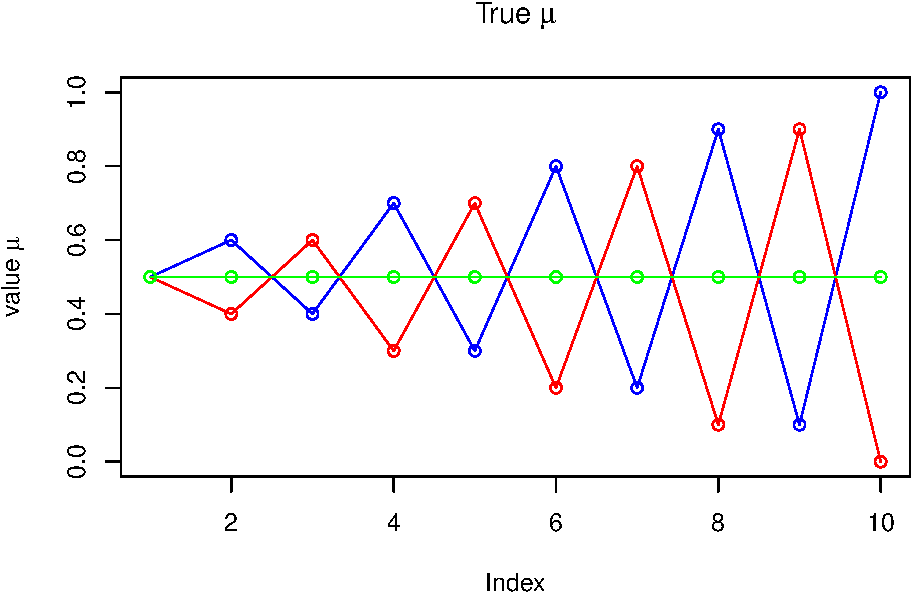
\includegraphics{MLLab1block2-lepeng_files/figure-latex/Assignment2_1-1.pdf}

\hypertarget{when-m3}{%
\subsection{when M=3}\label{when-m3}}

\begin{verbatim}
## [1] 0.3326090 0.3336558 0.3337352
\end{verbatim}

\begin{verbatim}
##           [,1]      [,2]      [,3]      [,4]      [,5]      [,6]      [,7]
## [1,] 0.4939877 0.4935375 0.5042511 0.5040286 0.4987810 0.5012754 0.4971036
## [2,] 0.4993719 0.5088453 0.5068730 0.5016720 0.4929275 0.5077146 0.5095075
## [3,] 0.4975302 0.5077926 0.4939841 0.5059821 0.5063490 0.5041462 0.4929400
##           [,8]      [,9]     [,10]
## [1,] 0.4982144 0.4987654 0.4929075
## [2,] 0.4924574 0.4992470 0.5008651
## [3,] 0.4992362 0.4943482 0.4903974
\end{verbatim}

\begin{verbatim}
## iteration:  1 log likelihood:  -6931.482
\end{verbatim}

\begin{verbatim}
## iteration:  2 log likelihood:  -6929.074
\end{verbatim}

\begin{verbatim}
## iteration:  3 log likelihood:  -6928.081
\end{verbatim}

\begin{verbatim}
## iteration:  4 log likelihood:  -6920.57
\end{verbatim}

\begin{verbatim}
## iteration:  5 log likelihood:  -6868.29
\end{verbatim}

\begin{verbatim}
## iteration:  6 log likelihood:  -6646.505
\end{verbatim}

\begin{verbatim}
## iteration:  7 log likelihood:  -6403.476
\end{verbatim}

\begin{verbatim}
## iteration:  8 log likelihood:  -6357.743
\end{verbatim}

\begin{verbatim}
## iteration:  9 log likelihood:  -6351.637
\end{verbatim}

\begin{verbatim}
## iteration:  10 log likelihood:  -6349.59
\end{verbatim}

\begin{verbatim}
## iteration:  11 log likelihood:  -6348.513
\end{verbatim}

\begin{verbatim}
## iteration:  12 log likelihood:  -6347.809
\end{verbatim}

\begin{verbatim}
## iteration:  13 log likelihood:  -6347.284
\end{verbatim}

\begin{verbatim}
## iteration:  14 log likelihood:  -6346.861
\end{verbatim}

\begin{verbatim}
## iteration:  15 log likelihood:  -6346.506
\end{verbatim}

\begin{verbatim}
## iteration:  16 log likelihood:  -6346.2
\end{verbatim}

\begin{verbatim}
## iteration:  17 log likelihood:  -6345.934
\end{verbatim}

\begin{verbatim}
## iteration:  18 log likelihood:  -6345.699
\end{verbatim}

\begin{verbatim}
## iteration:  19 log likelihood:  -6345.492
\end{verbatim}

\begin{verbatim}
## iteration:  20 log likelihood:  -6345.309
\end{verbatim}

\begin{verbatim}
## iteration:  21 log likelihood:  -6345.147
\end{verbatim}

\begin{verbatim}
## iteration:  22 log likelihood:  -6345.003
\end{verbatim}

\begin{verbatim}
## iteration:  23 log likelihood:  -6344.875
\end{verbatim}

\begin{verbatim}
## iteration:  24 log likelihood:  -6344.762
\end{verbatim}

\begin{verbatim}
## iteration:  25 log likelihood:  -6344.66
\end{verbatim}

\begin{verbatim}
## iteration:  26 log likelihood:  -6344.57
\end{verbatim}

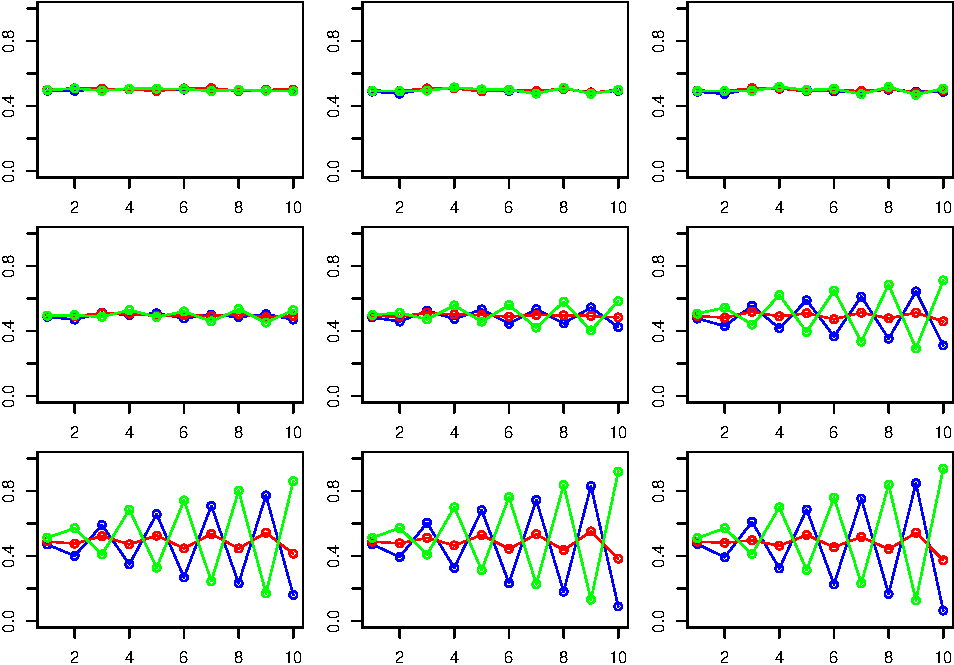
\includegraphics{MLLab1block2-lepeng_files/figure-latex/Assignment2_3-1.pdf}
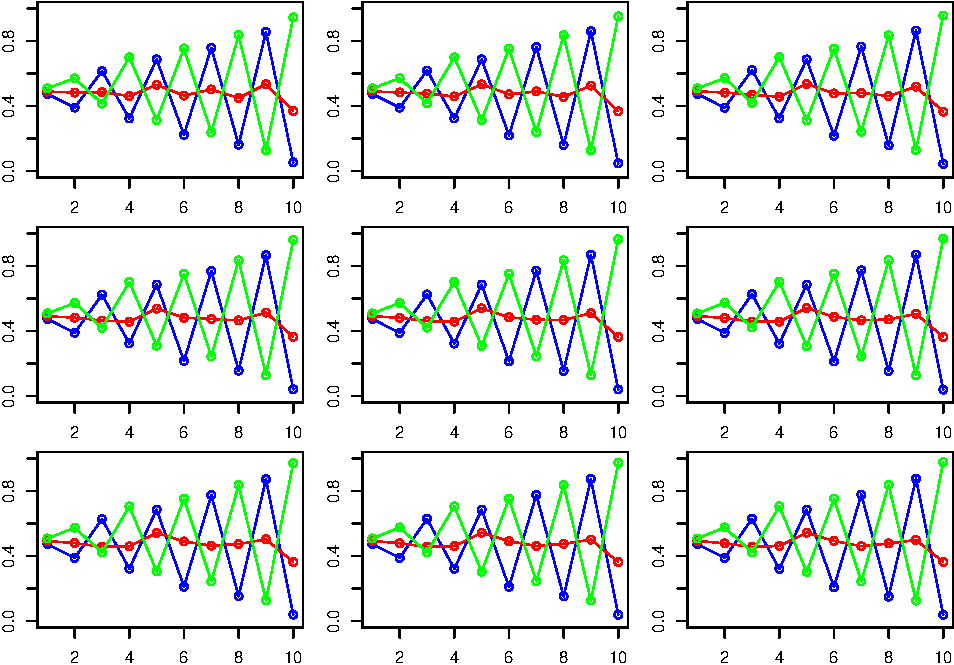
\includegraphics{MLLab1block2-lepeng_files/figure-latex/Assignment2_3-2.pdf}
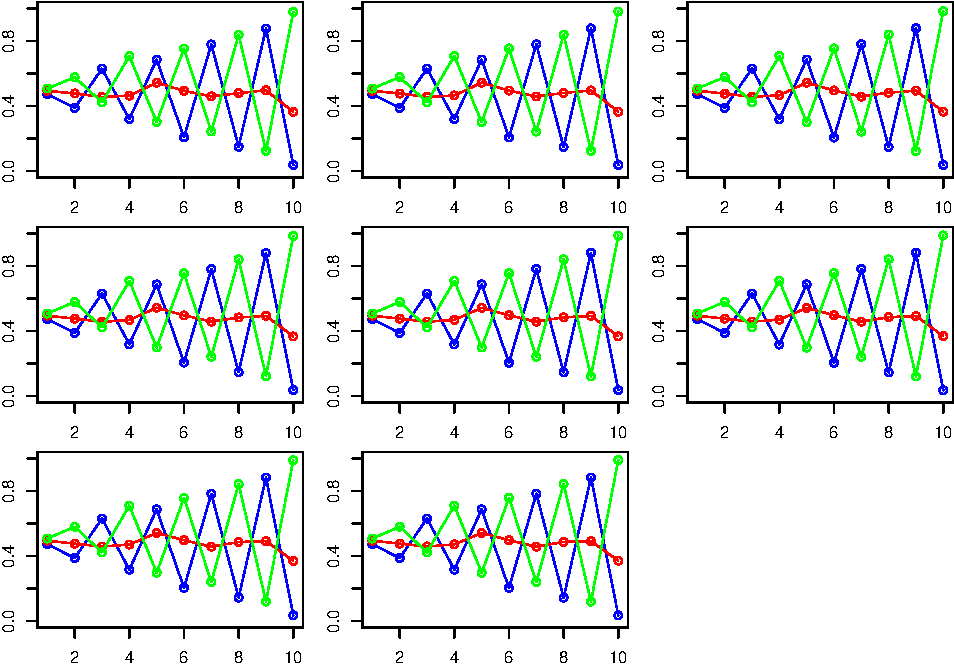
\includegraphics{MLLab1block2-lepeng_files/figure-latex/Assignment2_3-3.pdf}

\begin{verbatim}
## The final pi is:
\end{verbatim}

\begin{verbatim}
## [1] 0.3416794 0.2690298 0.3892909
\end{verbatim}

\begin{verbatim}
## The final mu is:
\end{verbatim}

\begin{verbatim}
##           [,1]      [,2]      [,3]      [,4]      [,5]      [,6]      [,7]
## [1,] 0.4727544 0.3869396 0.6302224 0.3156325 0.6875038 0.2030173 0.7832090
## [2,] 0.4939501 0.4757687 0.4584644 0.4711358 0.5413928 0.4976325 0.4569664
## [3,] 0.5075441 0.5800156 0.4221148 0.7100227 0.2965478 0.7571593 0.2400675
##           [,8]      [,9]      [,10]
## [1,] 0.1435650 0.8827796 0.03422816
## [2,] 0.4869015 0.4909904 0.37087402
## [3,] 0.8424441 0.1188864 0.99033611
\end{verbatim}

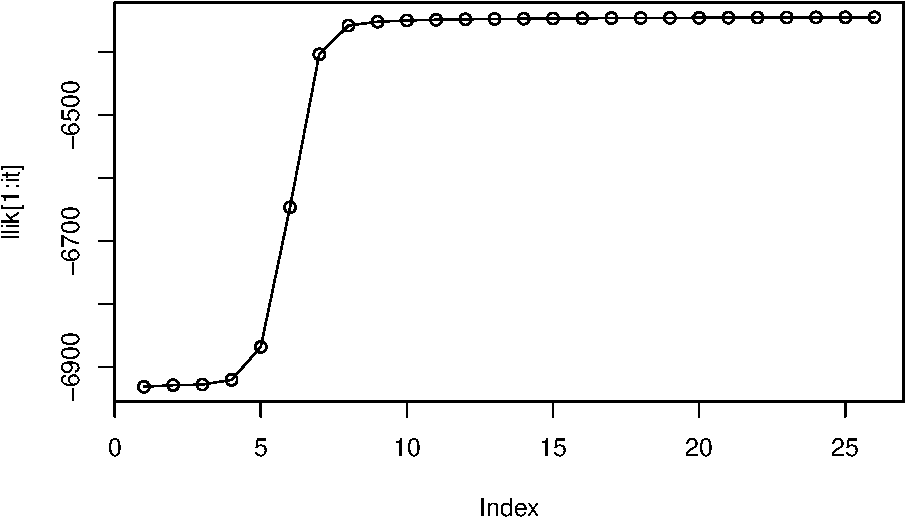
\includegraphics{MLLab1block2-lepeng_files/figure-latex/Assignment2_4-1.pdf}

\hypertarget{when-m2}{%
\subsection{when M=2}\label{when-m2}}

\begin{verbatim}
## [1] 0.5089877 0.4910123
\end{verbatim}

\begin{verbatim}
##           [,1]      [,2]      [,3]      [,4]      [,5]      [,6]      [,7]
## [1,] 0.4982342 0.4961948 0.4967226 0.4984220 0.4960055 0.4997165 0.5090205
## [2,] 0.4980423 0.5003773 0.5053941 0.4988233 0.4936057 0.4994058 0.4904128
##           [,8]      [,9]    [,10]
## [1,] 0.5057927 0.4947660 0.507127
## [2,] 0.5035921 0.4910555 0.494725
\end{verbatim}

\begin{verbatim}
## iteration:  1 log likelihood:  -6930.885
\end{verbatim}

\begin{verbatim}
## iteration:  2 log likelihood:  -6929.223
\end{verbatim}

\begin{verbatim}
## iteration:  3 log likelihood:  -6929.161
\end{verbatim}

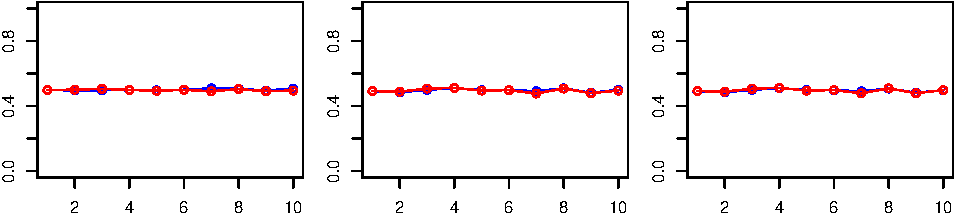
\includegraphics{MLLab1block2-lepeng_files/figure-latex/Assignment2_5-1.pdf}

\begin{verbatim}
## The final pi is:
\end{verbatim}

\begin{verbatim}
## [1] 0.5086338 0.4913662
\end{verbatim}

\begin{verbatim}
## The final mu is:
\end{verbatim}

\begin{verbatim}
##           [,1]      [,2]      [,3]      [,4]      [,5]      [,6]      [,7]
## [1,] 0.4918863 0.4840752 0.4997708 0.5100499 0.4974422 0.4976326 0.4900480
## [2,] 0.4921177 0.4879925 0.5063427 0.5119835 0.4945072 0.4983803 0.4777395
##           [,8]      [,9]     [,10]
## [1,] 0.5074063 0.4813071 0.4965251
## [2,] 0.5086146 0.4786470 0.4974916
\end{verbatim}

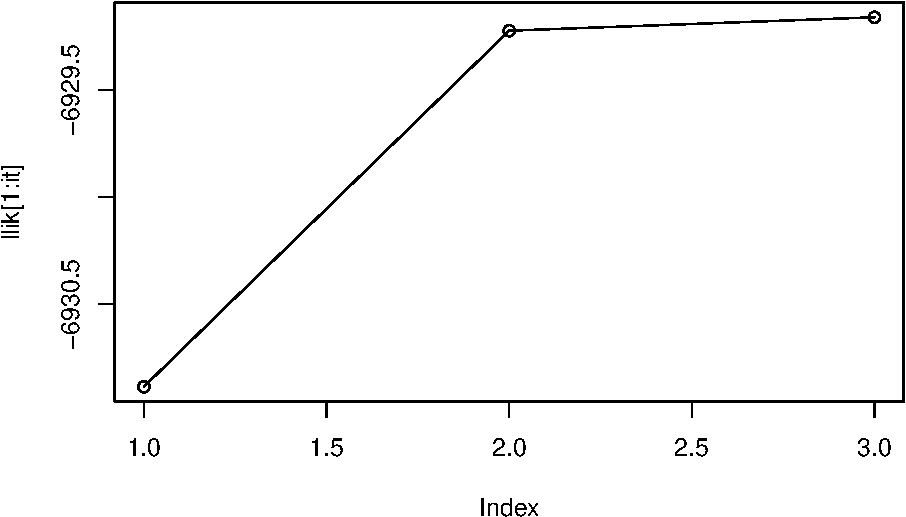
\includegraphics{MLLab1block2-lepeng_files/figure-latex/Assignment2_6-1.pdf}

\hypertarget{when-m4}{%
\subsection{when M=4}\label{when-m4}}

\begin{verbatim}
## [1] 0.2461659 0.2478605 0.2544456 0.2515279
\end{verbatim}

\begin{verbatim}
##           [,1]      [,2]      [,3]      [,4]      [,5]      [,6]      [,7]
## [1,] 0.4943551 0.5036051 0.4993455 0.5012054 0.5004571 0.4987214 0.4989227
## [2,] 0.5020358 0.5024204 0.5022187 0.4978065 0.5042903 0.5028750 0.4925821
## [3,] 0.4925133 0.4908125 0.4906579 0.4948314 0.4957019 0.4988231 0.4954166
## [4,] 0.4970116 0.4946235 0.5090379 0.5002896 0.5015360 0.4993958 0.4920966
##           [,8]      [,9]     [,10]
## [1,] 0.4917922 0.4954500 0.4901624
## [2,] 0.5086689 0.4947591 0.4942368
## [3,] 0.4925546 0.5016196 0.4978594
## [4,] 0.4947109 0.4902704 0.5019741
\end{verbatim}

\begin{verbatim}
## iteration:  1 log likelihood:  -6930.838
\end{verbatim}

\begin{verbatim}
## iteration:  2 log likelihood:  -6928.641
\end{verbatim}

\begin{verbatim}
## iteration:  3 log likelihood:  -6924.748
\end{verbatim}

\begin{verbatim}
## iteration:  4 log likelihood:  -6896.25
\end{verbatim}

\begin{verbatim}
## iteration:  5 log likelihood:  -6741.896
\end{verbatim}

\begin{verbatim}
## iteration:  6 log likelihood:  -6452.658
\end{verbatim}

\begin{verbatim}
## iteration:  7 log likelihood:  -6366.493
\end{verbatim}

\begin{verbatim}
## iteration:  8 log likelihood:  -6359.764
\end{verbatim}

\begin{verbatim}
## iteration:  9 log likelihood:  -6357.876
\end{verbatim}

\begin{verbatim}
## iteration:  10 log likelihood:  -6356.372
\end{verbatim}

\begin{verbatim}
## iteration:  11 log likelihood:  -6354.86
\end{verbatim}

\begin{verbatim}
## iteration:  12 log likelihood:  -6353.31
\end{verbatim}

\begin{verbatim}
## iteration:  13 log likelihood:  -6351.776
\end{verbatim}

\begin{verbatim}
## iteration:  14 log likelihood:  -6350.33
\end{verbatim}

\begin{verbatim}
## iteration:  15 log likelihood:  -6349.03
\end{verbatim}

\begin{verbatim}
## iteration:  16 log likelihood:  -6347.908
\end{verbatim}

\begin{verbatim}
## iteration:  17 log likelihood:  -6346.968
\end{verbatim}

\begin{verbatim}
## iteration:  18 log likelihood:  -6346.196
\end{verbatim}

\begin{verbatim}
## iteration:  19 log likelihood:  -6345.566
\end{verbatim}

\begin{verbatim}
## iteration:  20 log likelihood:  -6345.055
\end{verbatim}

\begin{verbatim}
## iteration:  21 log likelihood:  -6344.637
\end{verbatim}

\begin{verbatim}
## iteration:  22 log likelihood:  -6344.293
\end{verbatim}

\begin{verbatim}
## iteration:  23 log likelihood:  -6344.008
\end{verbatim}

\begin{verbatim}
## iteration:  24 log likelihood:  -6343.768
\end{verbatim}

\begin{verbatim}
## iteration:  25 log likelihood:  -6343.563
\end{verbatim}

\begin{verbatim}
## iteration:  26 log likelihood:  -6343.387
\end{verbatim}

\begin{verbatim}
## iteration:  27 log likelihood:  -6343.233
\end{verbatim}

\begin{verbatim}
## iteration:  28 log likelihood:  -6343.097
\end{verbatim}

\begin{verbatim}
## iteration:  29 log likelihood:  -6342.975
\end{verbatim}

\begin{verbatim}
## iteration:  30 log likelihood:  -6342.864
\end{verbatim}

\begin{verbatim}
## iteration:  31 log likelihood:  -6342.762
\end{verbatim}

\begin{verbatim}
## iteration:  32 log likelihood:  -6342.668
\end{verbatim}

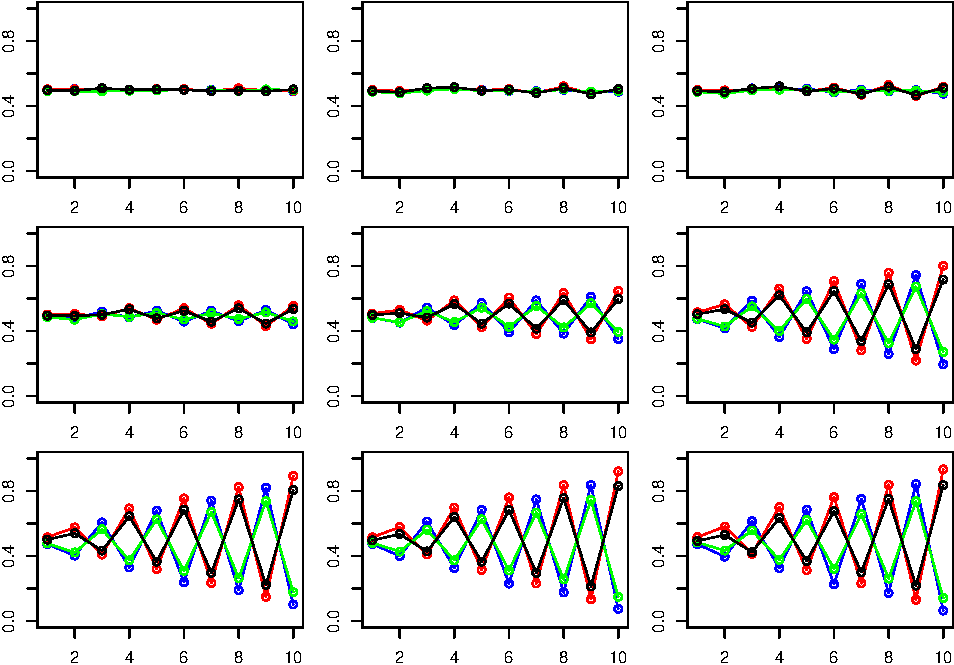
\includegraphics{MLLab1block2-lepeng_files/figure-latex/Assignment2_7-1.pdf}
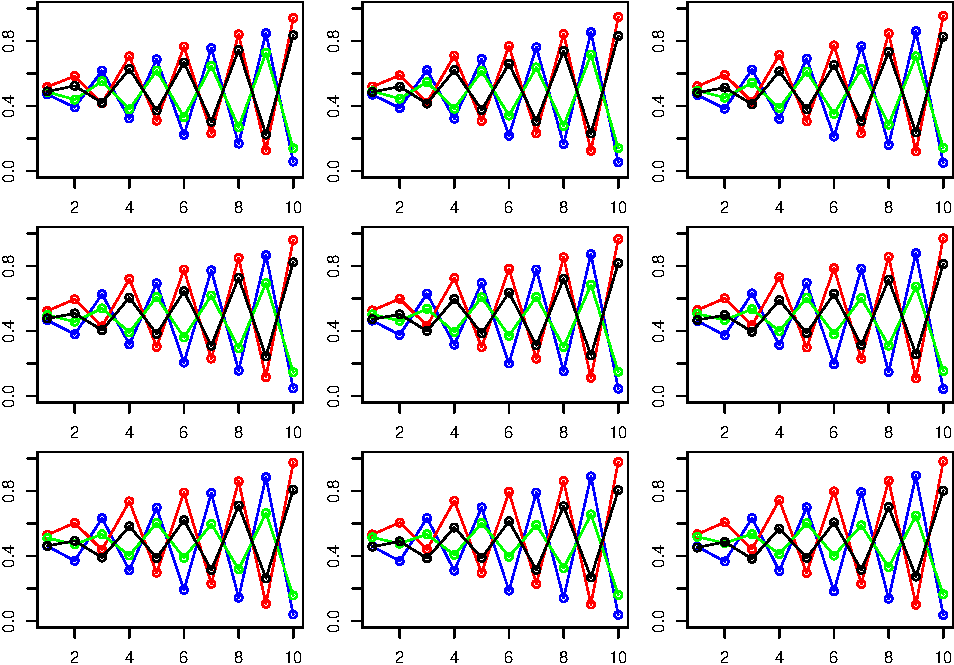
\includegraphics{MLLab1block2-lepeng_files/figure-latex/Assignment2_7-2.pdf}
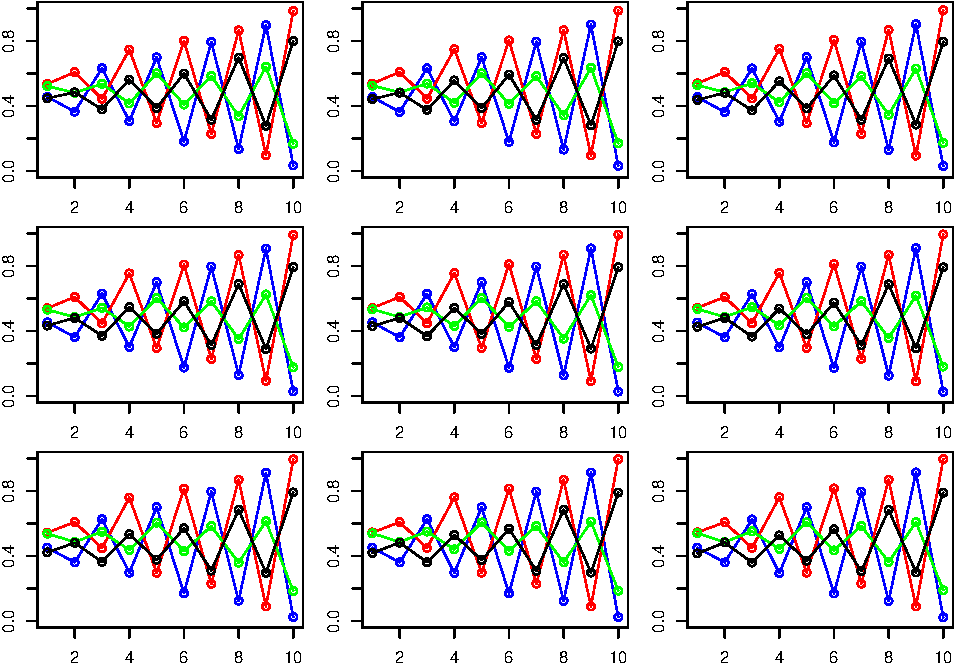
\includegraphics{MLLab1block2-lepeng_files/figure-latex/Assignment2_7-3.pdf}
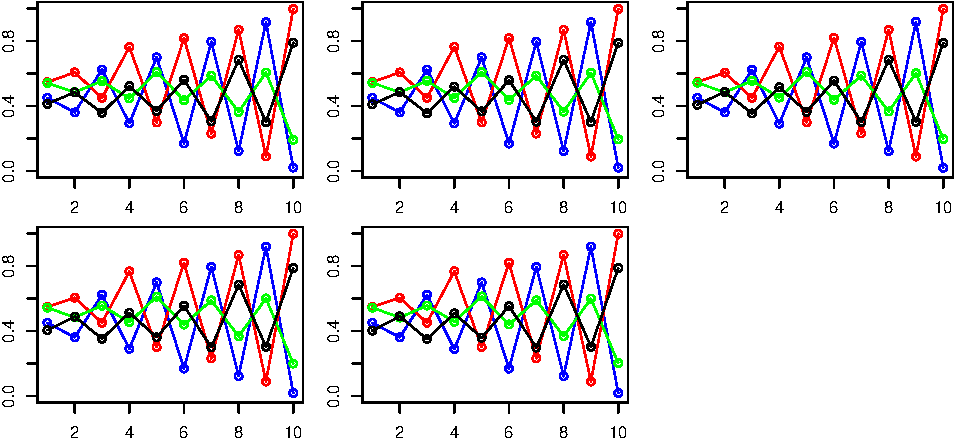
\includegraphics{MLLab1block2-lepeng_files/figure-latex/Assignment2_7-4.pdf}

\begin{verbatim}
## The final pi is:
\end{verbatim}

\begin{verbatim}
## [1] 0.2690190 0.2863050 0.2457246 0.1989515
\end{verbatim}

\begin{verbatim}
## The final mu is:
\end{verbatim}

\begin{verbatim}
##           [,1]      [,2]      [,3]      [,4]      [,5]      [,6]      [,7]
## [1,] 0.4502917 0.3606587 0.6220817 0.2892407 0.6986320 0.1681768 0.7943990
## [2,] 0.5487864 0.6040921 0.4511711 0.7675478 0.3010522 0.8195305 0.2318913
## [3,] 0.5439579 0.4827437 0.5563603 0.4568300 0.6123061 0.4400351 0.5885625
## [4,] 0.4025047 0.4895637 0.3506597 0.5085745 0.3588983 0.5528693 0.2979403
##           [,8]       [,9]      [,10]
## [1,] 0.1215732 0.91870837 0.01774129
## [2,] 0.8679302 0.08877946 0.99833984
## [3,] 0.3677877 0.59890299 0.20227253
## [4,] 0.6857315 0.30292227 0.78760041
\end{verbatim}

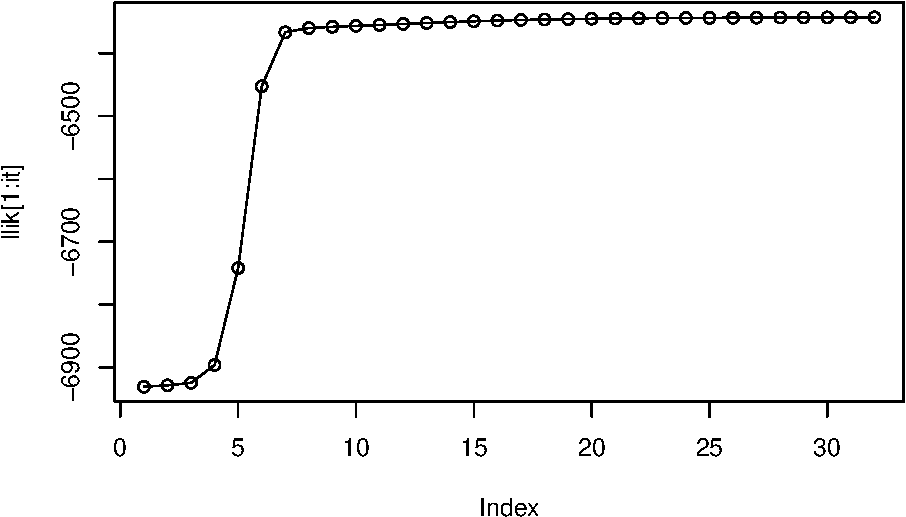
\includegraphics{MLLab1block2-lepeng_files/figure-latex/Assignment2_8-1.pdf}

According to above R results, it can be seen that:

\begin{enumerate}
\def\labelenumi{\arabic{enumi})}
\item
  When \(M=3\), the number of clusters in the model matches the true
  underlying structure of the data, thus in this scenario the estimated
  parameters can closely match the true mixing coefficients and
  conditional distributions(the final plot for \(\mu\) distribution are
  quite similar to the plot for true \(\mu\) distribution), and the
  model are able to capture the complexity of the data with three
  clusters. While, in terms of \(M=2\) or \(M=4\), the plots show that
  the estimated parameter deviate from the true distribution. When
  \(M=2\), the model oversimplify the data, leading to a less accurate
  representation of the true distribution. And when \(M=4\), the model
  try to fit into four clusters. As a result, the extra cluster might
  try to fit all the data, and overcomplicate the distribution. Besides,
  as the EM algorithm is for unsupervised learning, we don't the label
  each group orders for the training data, thus the order of final three
  clusters are not consistent with the order of true groups, but their
  distributions are similar.
\item
  According to the plots for log likelihood over iterations, when
  \(M=3\), the log likelihood increase steadily at the beginning, then
  reach a plateau after several iterations. The \(\mu\) distribution
  plots also align with such behavior.
\end{enumerate}

\hypertarget{appendix}{%
\section{Appendix}\label{appendix}}

\hypertarget{code-for-assignment-1}{%
\subsection{Code for Assignment 1}\label{code-for-assignment-1}}

\hypertarget{q1-1}{%
\subsubsection{Q1}\label{q1-1}}

\begin{Shaded}
\begin{Highlighting}[]
\FunctionTok{library}\NormalTok{(randomForest)}
\FunctionTok{library}\NormalTok{(knitr)}

\FunctionTok{set.seed}\NormalTok{(}\DecValTok{1234}\NormalTok{)}
\NormalTok{x1}\OtherTok{\textless{}{-}}\FunctionTok{runif}\NormalTok{(}\DecValTok{1000}\NormalTok{)}
\NormalTok{x2}\OtherTok{\textless{}{-}}\FunctionTok{runif}\NormalTok{(}\DecValTok{1000}\NormalTok{)}
\NormalTok{tedata}\OtherTok{\textless{}{-}}\FunctionTok{cbind}\NormalTok{(x1,x2)}
\NormalTok{y}\OtherTok{\textless{}{-}}\FunctionTok{as.numeric}\NormalTok{(x1}\SpecialCharTok{\textless{}}\NormalTok{x2)}
\NormalTok{telabels}\OtherTok{\textless{}{-}}\FunctionTok{as.factor}\NormalTok{(y)}
\CommentTok{\#plot(x1,x2,col=(y+1))}

\NormalTok{num\_tree }\OtherTok{\textless{}{-}} \FunctionTok{c}\NormalTok{(}\DecValTok{1}\NormalTok{,}\DecValTok{10}\NormalTok{,}\DecValTok{100}\NormalTok{)}
\NormalTok{num\_repeat }\OtherTok{\textless{}{-}} \DecValTok{1000}
\NormalTok{store\_mat }\OtherTok{\textless{}{-}} \FunctionTok{matrix}\NormalTok{(}\AttributeTok{nrow =}\NormalTok{ num\_repeat, }\AttributeTok{ncol =} \FunctionTok{length}\NormalTok{(num\_tree))}
\ControlFlowTok{for}\NormalTok{ (i }\ControlFlowTok{in} \DecValTok{1}\SpecialCharTok{:}\FunctionTok{length}\NormalTok{(num\_tree))\{}
  \ControlFlowTok{for}\NormalTok{ (j }\ControlFlowTok{in} \DecValTok{1}\SpecialCharTok{:}\NormalTok{num\_repeat)\{}
\NormalTok{    x1}\OtherTok{\textless{}{-}}\FunctionTok{runif}\NormalTok{(}\DecValTok{100}\NormalTok{)}
\NormalTok{    x2}\OtherTok{\textless{}{-}}\FunctionTok{runif}\NormalTok{(}\DecValTok{100}\NormalTok{)}
\NormalTok{    trdata}\OtherTok{\textless{}{-}}\FunctionTok{cbind}\NormalTok{(x1,x2)}
\NormalTok{    y}\OtherTok{\textless{}{-}}\FunctionTok{as.numeric}\NormalTok{(x1}\SpecialCharTok{\textless{}}\NormalTok{x2)}
\NormalTok{    trlabels}\OtherTok{\textless{}{-}}\FunctionTok{as.factor}\NormalTok{(y)}
    
\NormalTok{    m1 }\OtherTok{\textless{}{-}} \FunctionTok{randomForest}\NormalTok{(}\AttributeTok{x =}\NormalTok{ trdata, }\AttributeTok{y =}\NormalTok{ trlabels, }\AttributeTok{ntree =}\NormalTok{ num\_tree[i], }\AttributeTok{nodesize =} \DecValTok{25}\NormalTok{, }\AttributeTok{keep.forest =} \ConstantTok{TRUE}\NormalTok{)}
\NormalTok{    predicted\_labels }\OtherTok{\textless{}{-}} \FunctionTok{predict}\NormalTok{(m1, }\AttributeTok{newdata =}\NormalTok{ tedata)}
\NormalTok{    misclassification\_error }\OtherTok{\textless{}{-}} \FunctionTok{mean}\NormalTok{(predicted\_labels }\SpecialCharTok{!=}\NormalTok{ telabels)}
    
\NormalTok{    store\_mat[j,i] }\OtherTok{\textless{}{-}}\NormalTok{ misclassification\_error}
\NormalTok{  \}}
\NormalTok{\}}

\NormalTok{mean\_values }\OtherTok{\textless{}{-}} \FunctionTok{colMeans}\NormalTok{(store\_mat)}
\NormalTok{variance\_values }\OtherTok{\textless{}{-}} \FunctionTok{apply}\NormalTok{(store\_mat, }\DecValTok{2}\NormalTok{, var)}

\NormalTok{result\_df }\OtherTok{\textless{}{-}} \FunctionTok{data.frame}\NormalTok{(}\AttributeTok{Mean =}\NormalTok{ mean\_values, }\AttributeTok{Variance =}\NormalTok{ variance\_values)}
\FunctionTok{rownames}\NormalTok{(result\_df) }\OtherTok{\textless{}{-}} \FunctionTok{c}\NormalTok{(}\StringTok{"1 tree"}\NormalTok{, }\StringTok{"10 trees"}\NormalTok{, }\StringTok{"100 trees"}\NormalTok{)}
\FunctionTok{kable}\NormalTok{(result\_df, }\AttributeTok{caption =} \StringTok{"Classification Error"}\NormalTok{, }\AttributeTok{format =} \StringTok{"markdown"}\NormalTok{)}
\end{Highlighting}
\end{Shaded}

\hypertarget{q2-1}{%
\subsubsection{Q2}\label{q2-1}}

\begin{Shaded}
\begin{Highlighting}[]
\FunctionTok{set.seed}\NormalTok{(}\DecValTok{1234}\NormalTok{)}
\NormalTok{x1}\OtherTok{\textless{}{-}}\FunctionTok{runif}\NormalTok{(}\DecValTok{1000}\NormalTok{)}
\NormalTok{x2}\OtherTok{\textless{}{-}}\FunctionTok{runif}\NormalTok{(}\DecValTok{1000}\NormalTok{)}
\NormalTok{tedata}\OtherTok{\textless{}{-}}\FunctionTok{cbind}\NormalTok{(x1,x2)}
\NormalTok{y}\OtherTok{\textless{}{-}}\FunctionTok{as.numeric}\NormalTok{(x1}\SpecialCharTok{\textless{}}\FloatTok{0.5}\NormalTok{)}
\NormalTok{telabels}\OtherTok{\textless{}{-}}\FunctionTok{as.factor}\NormalTok{(y)}
\CommentTok{\#plot(x1,x2,col=(y+1))}

\NormalTok{num\_tree }\OtherTok{\textless{}{-}} \FunctionTok{c}\NormalTok{(}\DecValTok{1}\NormalTok{,}\DecValTok{10}\NormalTok{,}\DecValTok{100}\NormalTok{)}
\NormalTok{num\_repeat }\OtherTok{\textless{}{-}} \DecValTok{1000}
\NormalTok{store\_mat }\OtherTok{\textless{}{-}} \FunctionTok{matrix}\NormalTok{(}\AttributeTok{nrow =}\NormalTok{ num\_repeat, }\AttributeTok{ncol =} \FunctionTok{length}\NormalTok{(num\_tree))}
\ControlFlowTok{for}\NormalTok{ (i }\ControlFlowTok{in} \DecValTok{1}\SpecialCharTok{:}\FunctionTok{length}\NormalTok{(num\_tree))\{}
  \ControlFlowTok{for}\NormalTok{ (j }\ControlFlowTok{in} \DecValTok{1}\SpecialCharTok{:}\NormalTok{num\_repeat)\{}
\NormalTok{    x1}\OtherTok{\textless{}{-}}\FunctionTok{runif}\NormalTok{(}\DecValTok{100}\NormalTok{)}
\NormalTok{    x2}\OtherTok{\textless{}{-}}\FunctionTok{runif}\NormalTok{(}\DecValTok{100}\NormalTok{)}
\NormalTok{    trdata}\OtherTok{\textless{}{-}}\FunctionTok{cbind}\NormalTok{(x1,x2)}
\NormalTok{    y}\OtherTok{\textless{}{-}}\FunctionTok{as.numeric}\NormalTok{(x1}\SpecialCharTok{\textless{}}\FloatTok{0.5}\NormalTok{)}
\NormalTok{    trlabels}\OtherTok{\textless{}{-}}\FunctionTok{as.factor}\NormalTok{(y)}
    
\NormalTok{    m1 }\OtherTok{\textless{}{-}} \FunctionTok{randomForest}\NormalTok{(}\AttributeTok{x =}\NormalTok{ trdata, }\AttributeTok{y =}\NormalTok{ trlabels, }\AttributeTok{ntree =}\NormalTok{ num\_tree[i], }\AttributeTok{nodesize =} \DecValTok{25}\NormalTok{, }\AttributeTok{keep.forest =} \ConstantTok{TRUE}\NormalTok{)}
\NormalTok{    predicted\_labels }\OtherTok{\textless{}{-}} \FunctionTok{predict}\NormalTok{(m1, }\AttributeTok{newdata =}\NormalTok{ tedata)}
\NormalTok{    misclassification\_error }\OtherTok{\textless{}{-}} \FunctionTok{mean}\NormalTok{(predicted\_labels }\SpecialCharTok{!=}\NormalTok{ telabels)}
    
\NormalTok{    store\_mat[j,i] }\OtherTok{\textless{}{-}}\NormalTok{ misclassification\_error}
\NormalTok{  \}}
\NormalTok{\}}

\NormalTok{mean\_values }\OtherTok{\textless{}{-}} \FunctionTok{colMeans}\NormalTok{(store\_mat)}
\NormalTok{variance\_values }\OtherTok{\textless{}{-}} \FunctionTok{apply}\NormalTok{(store\_mat, }\DecValTok{2}\NormalTok{, var)}

\NormalTok{result\_df }\OtherTok{\textless{}{-}} \FunctionTok{data.frame}\NormalTok{(}\AttributeTok{Mean =}\NormalTok{ mean\_values, }\AttributeTok{Variance =}\NormalTok{ variance\_values)}
\FunctionTok{rownames}\NormalTok{(result\_df) }\OtherTok{\textless{}{-}} \FunctionTok{c}\NormalTok{(}\StringTok{"1 tree"}\NormalTok{, }\StringTok{"10 trees"}\NormalTok{, }\StringTok{"100 trees"}\NormalTok{)}
\FunctionTok{kable}\NormalTok{(result\_df, }\AttributeTok{caption =} \StringTok{"Classification Error"}\NormalTok{, }\AttributeTok{format =} \StringTok{"markdown"}\NormalTok{)}
\end{Highlighting}
\end{Shaded}

\hypertarget{q3-1}{%
\subsubsection{Q3}\label{q3-1}}

\begin{Shaded}
\begin{Highlighting}[]
\FunctionTok{set.seed}\NormalTok{(}\DecValTok{1234}\NormalTok{)}
\NormalTok{x1}\OtherTok{\textless{}{-}}\FunctionTok{runif}\NormalTok{(}\DecValTok{1000}\NormalTok{)}
\NormalTok{x2}\OtherTok{\textless{}{-}}\FunctionTok{runif}\NormalTok{(}\DecValTok{1000}\NormalTok{)}
\NormalTok{tedata}\OtherTok{\textless{}{-}}\FunctionTok{cbind}\NormalTok{(x1,x2)}
\NormalTok{y}\OtherTok{\textless{}{-}}\FunctionTok{as.numeric}\NormalTok{((x1}\SpecialCharTok{\textless{}}\FloatTok{0.5}\SpecialCharTok{\&}\NormalTok{x2}\SpecialCharTok{\textless{}}\FloatTok{0.5}\NormalTok{)}\SpecialCharTok{|}\NormalTok{(x1}\SpecialCharTok{\textgreater{}}\FloatTok{0.5}\SpecialCharTok{\&}\NormalTok{x2}\SpecialCharTok{\textgreater{}}\FloatTok{0.5}\NormalTok{))}
\NormalTok{telabels}\OtherTok{\textless{}{-}}\FunctionTok{as.factor}\NormalTok{(y)}
\CommentTok{\#plot(x1,x2,col=(y+1))}

\NormalTok{num\_tree }\OtherTok{\textless{}{-}} \FunctionTok{c}\NormalTok{(}\DecValTok{1}\NormalTok{,}\DecValTok{10}\NormalTok{,}\DecValTok{100}\NormalTok{)}
\NormalTok{num\_repeat }\OtherTok{\textless{}{-}} \DecValTok{1000}
\NormalTok{store\_mat }\OtherTok{\textless{}{-}} \FunctionTok{matrix}\NormalTok{(}\AttributeTok{nrow =}\NormalTok{ num\_repeat, }\AttributeTok{ncol =} \FunctionTok{length}\NormalTok{(num\_tree))}
\ControlFlowTok{for}\NormalTok{ (i }\ControlFlowTok{in} \DecValTok{1}\SpecialCharTok{:}\FunctionTok{length}\NormalTok{(num\_tree))\{}
  \ControlFlowTok{for}\NormalTok{ (j }\ControlFlowTok{in} \DecValTok{1}\SpecialCharTok{:}\NormalTok{num\_repeat)\{}
\NormalTok{    x1}\OtherTok{\textless{}{-}}\FunctionTok{runif}\NormalTok{(}\DecValTok{100}\NormalTok{)}
\NormalTok{    x2}\OtherTok{\textless{}{-}}\FunctionTok{runif}\NormalTok{(}\DecValTok{100}\NormalTok{)}
\NormalTok{    trdata}\OtherTok{\textless{}{-}}\FunctionTok{cbind}\NormalTok{(x1,x2)}
\NormalTok{    y}\OtherTok{\textless{}{-}}\FunctionTok{as.numeric}\NormalTok{((x1}\SpecialCharTok{\textless{}}\FloatTok{0.5}\SpecialCharTok{\&}\NormalTok{x2}\SpecialCharTok{\textless{}}\FloatTok{0.5}\NormalTok{)}\SpecialCharTok{|}\NormalTok{(x1}\SpecialCharTok{\textgreater{}}\FloatTok{0.5}\SpecialCharTok{\&}\NormalTok{x2}\SpecialCharTok{\textgreater{}}\FloatTok{0.5}\NormalTok{))}
\NormalTok{    trlabels}\OtherTok{\textless{}{-}}\FunctionTok{as.factor}\NormalTok{(y)}
    
\NormalTok{    m1 }\OtherTok{\textless{}{-}} \FunctionTok{randomForest}\NormalTok{(}\AttributeTok{x =}\NormalTok{ trdata, }\AttributeTok{y =}\NormalTok{ trlabels, }\AttributeTok{ntree =}\NormalTok{ num\_tree[i], }\AttributeTok{nodesize =} \DecValTok{12}\NormalTok{, }\AttributeTok{keep.forest =} \ConstantTok{TRUE}\NormalTok{)}
\NormalTok{    predicted\_labels }\OtherTok{\textless{}{-}} \FunctionTok{predict}\NormalTok{(m1, }\AttributeTok{newdata =}\NormalTok{ tedata)}
\NormalTok{    misclassification\_error }\OtherTok{\textless{}{-}} \FunctionTok{mean}\NormalTok{(predicted\_labels }\SpecialCharTok{!=}\NormalTok{ telabels)}
    
\NormalTok{    store\_mat[j,i] }\OtherTok{\textless{}{-}}\NormalTok{ misclassification\_error}
\NormalTok{  \}}
\NormalTok{\}}

\NormalTok{mean\_values }\OtherTok{\textless{}{-}} \FunctionTok{colMeans}\NormalTok{(store\_mat)}
\NormalTok{variance\_values }\OtherTok{\textless{}{-}} \FunctionTok{apply}\NormalTok{(store\_mat, }\DecValTok{2}\NormalTok{, var)}

\NormalTok{result\_df }\OtherTok{\textless{}{-}} \FunctionTok{data.frame}\NormalTok{(}\AttributeTok{Mean =}\NormalTok{ mean\_values, }\AttributeTok{Variance =}\NormalTok{ variance\_values)}
\FunctionTok{rownames}\NormalTok{(result\_df) }\OtherTok{\textless{}{-}} \FunctionTok{c}\NormalTok{(}\StringTok{"1 tree"}\NormalTok{, }\StringTok{"10 trees"}\NormalTok{, }\StringTok{"100 trees"}\NormalTok{)}
\FunctionTok{kable}\NormalTok{(result\_df, }\AttributeTok{caption =} \StringTok{"Classification Error"}\NormalTok{, }\AttributeTok{format =} \StringTok{"markdown"}\NormalTok{)}
\end{Highlighting}
\end{Shaded}

\hypertarget{code-for-assignment-2}{%
\subsection{Code for Assignment 2}\label{code-for-assignment-2}}

\begin{Shaded}
\begin{Highlighting}[]
\FunctionTok{set.seed}\NormalTok{(}\DecValTok{1234567890}\NormalTok{)}
\NormalTok{max\_it }\OtherTok{\textless{}{-}} \DecValTok{100} \CommentTok{\# max number of EM iterations}
\NormalTok{min\_change }\OtherTok{\textless{}{-}} \FloatTok{0.1} \CommentTok{\# min change in log lik between two consecutive iterations}
\NormalTok{n}\OtherTok{=}\DecValTok{1000} \CommentTok{\# number of training points}
\NormalTok{D}\OtherTok{=}\DecValTok{10} \CommentTok{\# number of dimensions}
\NormalTok{x }\OtherTok{\textless{}{-}} \FunctionTok{matrix}\NormalTok{(}\AttributeTok{nrow=}\NormalTok{n, }\AttributeTok{ncol=}\NormalTok{D) }\CommentTok{\# training data}
\NormalTok{true\_pi }\OtherTok{\textless{}{-}} \FunctionTok{vector}\NormalTok{(}\AttributeTok{length =} \DecValTok{3}\NormalTok{) }\CommentTok{\# true mixing coefficients}
\NormalTok{true\_mu }\OtherTok{\textless{}{-}} \FunctionTok{matrix}\NormalTok{(}\AttributeTok{nrow=}\DecValTok{3}\NormalTok{, }\AttributeTok{ncol=}\NormalTok{D) }\CommentTok{\# true conditional distributions}
\NormalTok{true\_pi}\OtherTok{=}\FunctionTok{c}\NormalTok{(}\DecValTok{1}\SpecialCharTok{/}\DecValTok{3}\NormalTok{, }\DecValTok{1}\SpecialCharTok{/}\DecValTok{3}\NormalTok{, }\DecValTok{1}\SpecialCharTok{/}\DecValTok{3}\NormalTok{)}
\NormalTok{true\_mu[}\DecValTok{1}\NormalTok{,]}\OtherTok{=}\FunctionTok{c}\NormalTok{(}\FloatTok{0.5}\NormalTok{,}\FloatTok{0.6}\NormalTok{,}\FloatTok{0.4}\NormalTok{,}\FloatTok{0.7}\NormalTok{,}\FloatTok{0.3}\NormalTok{,}\FloatTok{0.8}\NormalTok{,}\FloatTok{0.2}\NormalTok{,}\FloatTok{0.9}\NormalTok{,}\FloatTok{0.1}\NormalTok{,}\DecValTok{1}\NormalTok{)}
\NormalTok{true\_mu[}\DecValTok{2}\NormalTok{,]}\OtherTok{=}\FunctionTok{c}\NormalTok{(}\FloatTok{0.5}\NormalTok{,}\FloatTok{0.4}\NormalTok{,}\FloatTok{0.6}\NormalTok{,}\FloatTok{0.3}\NormalTok{,}\FloatTok{0.7}\NormalTok{,}\FloatTok{0.2}\NormalTok{,}\FloatTok{0.8}\NormalTok{,}\FloatTok{0.1}\NormalTok{,}\FloatTok{0.9}\NormalTok{,}\DecValTok{0}\NormalTok{)}
\NormalTok{true\_mu[}\DecValTok{3}\NormalTok{,]}\OtherTok{=}\FunctionTok{c}\NormalTok{(}\FloatTok{0.5}\NormalTok{,}\FloatTok{0.5}\NormalTok{,}\FloatTok{0.5}\NormalTok{,}\FloatTok{0.5}\NormalTok{,}\FloatTok{0.5}\NormalTok{,}\FloatTok{0.5}\NormalTok{,}\FloatTok{0.5}\NormalTok{,}\FloatTok{0.5}\NormalTok{,}\FloatTok{0.5}\NormalTok{,}\FloatTok{0.5}\NormalTok{)}
\FunctionTok{plot}\NormalTok{(true\_mu[}\DecValTok{1}\NormalTok{,], }\AttributeTok{type=}\StringTok{"o"}\NormalTok{, }\AttributeTok{col=}\StringTok{"blue"}\NormalTok{, }\AttributeTok{ylim=}\FunctionTok{c}\NormalTok{(}\DecValTok{0}\NormalTok{,}\DecValTok{1}\NormalTok{), }\AttributeTok{ylab =} \FunctionTok{expression}\NormalTok{(}\StringTok{"value "}\SpecialCharTok{*}\NormalTok{mu), }\AttributeTok{main =} \FunctionTok{expression}\NormalTok{(}\StringTok{"True "} \SpecialCharTok{*}\NormalTok{ mu))}
\FunctionTok{points}\NormalTok{(true\_mu[}\DecValTok{2}\NormalTok{,], }\AttributeTok{type=}\StringTok{"o"}\NormalTok{, }\AttributeTok{col=}\StringTok{"red"}\NormalTok{)}
\FunctionTok{points}\NormalTok{(true\_mu[}\DecValTok{3}\NormalTok{,], }\AttributeTok{type=}\StringTok{"o"}\NormalTok{, }\AttributeTok{col=}\StringTok{"green"}\NormalTok{)}
\CommentTok{\#legend("bottomleft", legend = c(expression(mu[1]), expression(mu[2]), expression(mu[3])), col = c("blue", "red", "green"), pch = 1, bty = "n")}

\CommentTok{\# Producing the training data}
\ControlFlowTok{for}\NormalTok{(i }\ControlFlowTok{in} \DecValTok{1}\SpecialCharTok{:}\NormalTok{n) \{}
\NormalTok{  m }\OtherTok{\textless{}{-}} \FunctionTok{sample}\NormalTok{(}\DecValTok{1}\SpecialCharTok{:}\DecValTok{3}\NormalTok{,}\DecValTok{1}\NormalTok{,}\AttributeTok{prob=}\NormalTok{true\_pi)}
  \ControlFlowTok{for}\NormalTok{(d }\ControlFlowTok{in} \DecValTok{1}\SpecialCharTok{:}\NormalTok{D) \{}
\NormalTok{    x[i,d] }\OtherTok{\textless{}{-}} \FunctionTok{rbinom}\NormalTok{(}\DecValTok{1}\NormalTok{,}\DecValTok{1}\NormalTok{,true\_mu[m,d])}
\NormalTok{  \}}
\NormalTok{\}}
\end{Highlighting}
\end{Shaded}

\hypertarget{when-m3-1}{%
\subsubsection{when M=3}\label{when-m3-1}}

\begin{Shaded}
\begin{Highlighting}[]
\NormalTok{M}\OtherTok{=}\DecValTok{3} \CommentTok{\# number of clusters}
\NormalTok{w }\OtherTok{\textless{}{-}} \FunctionTok{matrix}\NormalTok{(}\AttributeTok{nrow=}\NormalTok{n, }\AttributeTok{ncol=}\NormalTok{M) }\CommentTok{\# weights}
\NormalTok{pi }\OtherTok{\textless{}{-}} \FunctionTok{vector}\NormalTok{(}\AttributeTok{length =}\NormalTok{ M) }\CommentTok{\# mixing coefficients}
\NormalTok{mu }\OtherTok{\textless{}{-}} \FunctionTok{matrix}\NormalTok{(}\AttributeTok{nrow=}\NormalTok{M, }\AttributeTok{ncol=}\NormalTok{D) }\CommentTok{\# conditional distributions}
\NormalTok{llik }\OtherTok{\textless{}{-}} \FunctionTok{vector}\NormalTok{(}\AttributeTok{length =}\NormalTok{ max\_it) }\CommentTok{\# log likelihood of the EM iterations}
\CommentTok{\# Random initialization of the parameters}
\NormalTok{pi }\OtherTok{\textless{}{-}} \FunctionTok{runif}\NormalTok{(M,}\FloatTok{0.49}\NormalTok{,}\FloatTok{0.51}\NormalTok{)}
\NormalTok{pi }\OtherTok{\textless{}{-}}\NormalTok{ pi }\SpecialCharTok{/} \FunctionTok{sum}\NormalTok{(pi)}
\ControlFlowTok{for}\NormalTok{(m }\ControlFlowTok{in} \DecValTok{1}\SpecialCharTok{:}\NormalTok{M) \{}
\NormalTok{  mu[m,] }\OtherTok{\textless{}{-}} \FunctionTok{runif}\NormalTok{(D,}\FloatTok{0.49}\NormalTok{,}\FloatTok{0.51}\NormalTok{)}
\NormalTok{\}}
\NormalTok{pi}
\NormalTok{mu}

\CommentTok{\# create this vector to store value}
\NormalTok{w\_sum }\OtherTok{\textless{}{-}} \FunctionTok{vector}\NormalTok{(}\AttributeTok{length =}\NormalTok{ n)}
\CommentTok{\# make labels and margins smaller}
\FunctionTok{par}\NormalTok{(}\AttributeTok{cex=}\FloatTok{0.8}\NormalTok{, }\AttributeTok{mar=}\FunctionTok{c}\NormalTok{(}\DecValTok{2}\NormalTok{,}\DecValTok{2}\NormalTok{,}\FloatTok{0.5}\NormalTok{,}\DecValTok{1}\NormalTok{), }\AttributeTok{mfrow =} \FunctionTok{c}\NormalTok{(}\DecValTok{3}\NormalTok{, }\DecValTok{3}\NormalTok{))}

\ControlFlowTok{for}\NormalTok{(it }\ControlFlowTok{in} \DecValTok{1}\SpecialCharTok{:}\NormalTok{max\_it) \{}
  \FunctionTok{plot}\NormalTok{(mu[}\DecValTok{1}\NormalTok{,], }\AttributeTok{type=}\StringTok{"o"}\NormalTok{, }\AttributeTok{col=}\StringTok{"blue"}\NormalTok{, }\AttributeTok{ylim=}\FunctionTok{c}\NormalTok{(}\DecValTok{0}\NormalTok{,}\DecValTok{1}\NormalTok{), }\AttributeTok{ylab =} \FunctionTok{expression}\NormalTok{(}\StringTok{"value "}\SpecialCharTok{*}\NormalTok{mu))}
  \FunctionTok{points}\NormalTok{(mu[}\DecValTok{2}\NormalTok{,], }\AttributeTok{type=}\StringTok{"o"}\NormalTok{, }\AttributeTok{col=}\StringTok{"red"}\NormalTok{)}
  \FunctionTok{points}\NormalTok{(mu[}\DecValTok{3}\NormalTok{,], }\AttributeTok{type=}\StringTok{"o"}\NormalTok{, }\AttributeTok{col=}\StringTok{"green"}\NormalTok{)}
  \CommentTok{\#points(mu[4,], type="o", col="yellow")}
  \FunctionTok{Sys.sleep}\NormalTok{(}\FloatTok{0.5}\NormalTok{)}
  \CommentTok{\# E{-}step: Computation of the weights}
  \ControlFlowTok{for}\NormalTok{ (i }\ControlFlowTok{in} \DecValTok{1}\SpecialCharTok{:}\NormalTok{n) \{}
    \ControlFlowTok{for}\NormalTok{ (m }\ControlFlowTok{in} \DecValTok{1}\SpecialCharTok{:}\NormalTok{M) \{}
      \CommentTok{\# log operation for convenience}
\NormalTok{      w[i, m] }\OtherTok{\textless{}{-}} \FunctionTok{log}\NormalTok{(pi[m]) }\SpecialCharTok{+} \FunctionTok{sum}\NormalTok{(x[i, ] }\SpecialCharTok{*} \FunctionTok{log}\NormalTok{(mu[m, ]) }\SpecialCharTok{+}\NormalTok{ (}\DecValTok{1} \SpecialCharTok{{-}}\NormalTok{ x[i, ]) }\SpecialCharTok{*} \FunctionTok{log}\NormalTok{(}\DecValTok{1} \SpecialCharTok{{-}}\NormalTok{ mu[m, ]))}
\NormalTok{    \}}
    \CommentTok{\# exp operation for setting value back}
\NormalTok{    w[i, ] }\OtherTok{\textless{}{-}} \FunctionTok{exp}\NormalTok{(w[i, ])}
    \CommentTok{\# get the real w[i,m]}
\NormalTok{    w\_sum[i] }\OtherTok{\textless{}{-}} \FunctionTok{sum}\NormalTok{(w[i, ])}
\NormalTok{    w[i, ] }\OtherTok{\textless{}{-}}\NormalTok{ w[i, ] }\SpecialCharTok{/}\NormalTok{ w\_sum[i]}
\NormalTok{  \}}
  \CommentTok{\#Log likelihood computation.}
\NormalTok{  llik[it] }\OtherTok{\textless{}{-}} \FunctionTok{sum}\NormalTok{(}\FunctionTok{log}\NormalTok{(w\_sum))}
  
  \FunctionTok{cat}\NormalTok{(}\StringTok{"iteration: "}\NormalTok{, it, }\StringTok{"log likelihood: "}\NormalTok{, llik[it], }\StringTok{"}\SpecialCharTok{\textbackslash{}n}\StringTok{"}\NormalTok{)}
  \FunctionTok{flush.console}\NormalTok{()}
  \CommentTok{\# Stop if the lok likelihood has not changed significantly}
  \ControlFlowTok{if}\NormalTok{ (it }\SpecialCharTok{\textgreater{}} \DecValTok{1} \SpecialCharTok{\&\&} \FunctionTok{abs}\NormalTok{(llik[it] }\SpecialCharTok{{-}}\NormalTok{ llik[it }\SpecialCharTok{{-}} \DecValTok{1}\NormalTok{]) }\SpecialCharTok{\textless{}}\NormalTok{ min\_change) \{}
    \ControlFlowTok{break}
\NormalTok{  \}}
  \CommentTok{\#M{-}step: ML parameter estimation from the data and weights}
\NormalTok{  pi }\OtherTok{\textless{}{-}} \FunctionTok{colMeans}\NormalTok{(w)}
  \ControlFlowTok{for}\NormalTok{ (m }\ControlFlowTok{in} \DecValTok{1}\SpecialCharTok{:}\NormalTok{M) \{}
\NormalTok{    mu[m, ] }\OtherTok{\textless{}{-}} \FunctionTok{colSums}\NormalTok{(w[, m] }\SpecialCharTok{*}\NormalTok{ x) }\SpecialCharTok{/} \FunctionTok{sum}\NormalTok{(w[, m])}
\NormalTok{  \}}
\NormalTok{\}}

\FunctionTok{cat}\NormalTok{(}\StringTok{"The final pi is:}\SpecialCharTok{\textbackslash{}n}\StringTok{"}\NormalTok{)}
\NormalTok{pi}
\FunctionTok{cat}\NormalTok{(}\StringTok{"The final mu is:}\SpecialCharTok{\textbackslash{}n}\StringTok{"}\NormalTok{)}
\NormalTok{mu}
\FunctionTok{plot}\NormalTok{(llik[}\DecValTok{1}\SpecialCharTok{:}\NormalTok{it], }\AttributeTok{type=}\StringTok{"o"}\NormalTok{)}
\end{Highlighting}
\end{Shaded}

\hypertarget{when-m2-1}{%
\subsubsection{when M=2}\label{when-m2-1}}

\begin{Shaded}
\begin{Highlighting}[]
\NormalTok{M}\OtherTok{=}\DecValTok{2} \CommentTok{\# number of clusters}
\NormalTok{w }\OtherTok{\textless{}{-}} \FunctionTok{matrix}\NormalTok{(}\AttributeTok{nrow=}\NormalTok{n, }\AttributeTok{ncol=}\NormalTok{M) }\CommentTok{\# weights}
\NormalTok{pi }\OtherTok{\textless{}{-}} \FunctionTok{vector}\NormalTok{(}\AttributeTok{length =}\NormalTok{ M) }\CommentTok{\# mixing coefficients}
\NormalTok{mu }\OtherTok{\textless{}{-}} \FunctionTok{matrix}\NormalTok{(}\AttributeTok{nrow=}\NormalTok{M, }\AttributeTok{ncol=}\NormalTok{D) }\CommentTok{\# conditional distributions}
\NormalTok{llik }\OtherTok{\textless{}{-}} \FunctionTok{vector}\NormalTok{(}\AttributeTok{length =}\NormalTok{ max\_it) }\CommentTok{\# log likelihood of the EM iterations}
\CommentTok{\# Random initialization of the parameters}
\NormalTok{pi }\OtherTok{\textless{}{-}} \FunctionTok{runif}\NormalTok{(M,}\FloatTok{0.49}\NormalTok{,}\FloatTok{0.51}\NormalTok{)}
\NormalTok{pi }\OtherTok{\textless{}{-}}\NormalTok{ pi }\SpecialCharTok{/} \FunctionTok{sum}\NormalTok{(pi)}
\ControlFlowTok{for}\NormalTok{(m }\ControlFlowTok{in} \DecValTok{1}\SpecialCharTok{:}\NormalTok{M) \{}
\NormalTok{  mu[m,] }\OtherTok{\textless{}{-}} \FunctionTok{runif}\NormalTok{(D,}\FloatTok{0.49}\NormalTok{,}\FloatTok{0.51}\NormalTok{)}
\NormalTok{\}}
\NormalTok{pi}
\NormalTok{mu}

\CommentTok{\# create this vector to store value}
\NormalTok{w\_sum }\OtherTok{\textless{}{-}} \FunctionTok{vector}\NormalTok{(}\AttributeTok{length =}\NormalTok{ n)}
\CommentTok{\# make labels and margins smaller}
\FunctionTok{par}\NormalTok{(}\AttributeTok{cex=}\FloatTok{0.8}\NormalTok{, }\AttributeTok{mar=}\FunctionTok{c}\NormalTok{(}\DecValTok{2}\NormalTok{,}\DecValTok{2}\NormalTok{,}\FloatTok{0.5}\NormalTok{,}\DecValTok{1}\NormalTok{), }\AttributeTok{mfrow =} \FunctionTok{c}\NormalTok{(}\DecValTok{3}\NormalTok{, }\DecValTok{3}\NormalTok{))}

\ControlFlowTok{for}\NormalTok{(it }\ControlFlowTok{in} \DecValTok{1}\SpecialCharTok{:}\NormalTok{max\_it) \{}
  \FunctionTok{plot}\NormalTok{(mu[}\DecValTok{1}\NormalTok{,], }\AttributeTok{type=}\StringTok{"o"}\NormalTok{, }\AttributeTok{col=}\StringTok{"blue"}\NormalTok{, }\AttributeTok{ylim=}\FunctionTok{c}\NormalTok{(}\DecValTok{0}\NormalTok{,}\DecValTok{1}\NormalTok{), }\AttributeTok{ylab =} \FunctionTok{expression}\NormalTok{(}\StringTok{"value "}\SpecialCharTok{*}\NormalTok{mu))}
  \FunctionTok{points}\NormalTok{(mu[}\DecValTok{2}\NormalTok{,], }\AttributeTok{type=}\StringTok{"o"}\NormalTok{, }\AttributeTok{col=}\StringTok{"red"}\NormalTok{)}
 \CommentTok{\# points(mu[3,], type="o", col="green")}
  \CommentTok{\#points(mu[4,], type="o", col="yellow")}
  \FunctionTok{Sys.sleep}\NormalTok{(}\FloatTok{0.5}\NormalTok{)}
  \CommentTok{\# E{-}step: Computation of the weights}
  \ControlFlowTok{for}\NormalTok{ (i }\ControlFlowTok{in} \DecValTok{1}\SpecialCharTok{:}\NormalTok{n) \{}
    \ControlFlowTok{for}\NormalTok{ (m }\ControlFlowTok{in} \DecValTok{1}\SpecialCharTok{:}\NormalTok{M) \{}
      \CommentTok{\# log operation for convenience}
\NormalTok{      w[i, m] }\OtherTok{\textless{}{-}} \FunctionTok{log}\NormalTok{(pi[m]) }\SpecialCharTok{+} \FunctionTok{sum}\NormalTok{(x[i, ] }\SpecialCharTok{*} \FunctionTok{log}\NormalTok{(mu[m, ]) }\SpecialCharTok{+}\NormalTok{ (}\DecValTok{1} \SpecialCharTok{{-}}\NormalTok{ x[i, ]) }\SpecialCharTok{*} \FunctionTok{log}\NormalTok{(}\DecValTok{1} \SpecialCharTok{{-}}\NormalTok{ mu[m, ]))}
\NormalTok{    \}}
    \CommentTok{\# exp operation for setting value back}
\NormalTok{    w[i, ] }\OtherTok{\textless{}{-}} \FunctionTok{exp}\NormalTok{(w[i, ])}
    \CommentTok{\# get the real w[i,m]}
\NormalTok{    w\_sum[i] }\OtherTok{\textless{}{-}} \FunctionTok{sum}\NormalTok{(w[i, ])}
\NormalTok{    w[i, ] }\OtherTok{\textless{}{-}}\NormalTok{ w[i, ] }\SpecialCharTok{/}\NormalTok{ w\_sum[i]}
\NormalTok{  \}}
  \CommentTok{\#Log likelihood computation.}
\NormalTok{  llik[it] }\OtherTok{\textless{}{-}} \FunctionTok{sum}\NormalTok{(}\FunctionTok{log}\NormalTok{(w\_sum))}
  
  \FunctionTok{cat}\NormalTok{(}\StringTok{"iteration: "}\NormalTok{, it, }\StringTok{"log likelihood: "}\NormalTok{, llik[it], }\StringTok{"}\SpecialCharTok{\textbackslash{}n}\StringTok{"}\NormalTok{)}
  \FunctionTok{flush.console}\NormalTok{()}
  \CommentTok{\# Stop if the lok likelihood has not changed significantly}
  \ControlFlowTok{if}\NormalTok{ (it }\SpecialCharTok{\textgreater{}} \DecValTok{1} \SpecialCharTok{\&\&} \FunctionTok{abs}\NormalTok{(llik[it] }\SpecialCharTok{{-}}\NormalTok{ llik[it }\SpecialCharTok{{-}} \DecValTok{1}\NormalTok{]) }\SpecialCharTok{\textless{}}\NormalTok{ min\_change) \{}
    \ControlFlowTok{break}
\NormalTok{  \}}
  \CommentTok{\#M{-}step: ML parameter estimation from the data and weights}
\NormalTok{  pi }\OtherTok{\textless{}{-}} \FunctionTok{colMeans}\NormalTok{(w)}
  \ControlFlowTok{for}\NormalTok{ (m }\ControlFlowTok{in} \DecValTok{1}\SpecialCharTok{:}\NormalTok{M) \{}
\NormalTok{    mu[m, ] }\OtherTok{\textless{}{-}} \FunctionTok{colSums}\NormalTok{(w[, m] }\SpecialCharTok{*}\NormalTok{ x) }\SpecialCharTok{/} \FunctionTok{sum}\NormalTok{(w[, m])}
\NormalTok{  \}}
\NormalTok{\}}

\FunctionTok{cat}\NormalTok{(}\StringTok{"The final pi is:}\SpecialCharTok{\textbackslash{}n}\StringTok{"}\NormalTok{)}
\NormalTok{pi}
\FunctionTok{cat}\NormalTok{(}\StringTok{"The final mu is:}\SpecialCharTok{\textbackslash{}n}\StringTok{"}\NormalTok{)}
\NormalTok{mu}
\FunctionTok{plot}\NormalTok{(llik[}\DecValTok{1}\SpecialCharTok{:}\NormalTok{it], }\AttributeTok{type=}\StringTok{"o"}\NormalTok{)}
\end{Highlighting}
\end{Shaded}

\hypertarget{when-m4-1}{%
\subsubsection{when M=4}\label{when-m4-1}}

\begin{Shaded}
\begin{Highlighting}[]
\NormalTok{M}\OtherTok{=}\DecValTok{4} \CommentTok{\# number of clusters}
\NormalTok{w }\OtherTok{\textless{}{-}} \FunctionTok{matrix}\NormalTok{(}\AttributeTok{nrow=}\NormalTok{n, }\AttributeTok{ncol=}\NormalTok{M) }\CommentTok{\# weights}
\NormalTok{pi }\OtherTok{\textless{}{-}} \FunctionTok{vector}\NormalTok{(}\AttributeTok{length =}\NormalTok{ M) }\CommentTok{\# mixing coefficients}
\NormalTok{mu }\OtherTok{\textless{}{-}} \FunctionTok{matrix}\NormalTok{(}\AttributeTok{nrow=}\NormalTok{M, }\AttributeTok{ncol=}\NormalTok{D) }\CommentTok{\# conditional distributions}
\NormalTok{llik }\OtherTok{\textless{}{-}} \FunctionTok{vector}\NormalTok{(}\AttributeTok{length =}\NormalTok{ max\_it) }\CommentTok{\# log likelihood of the EM iterations}
\CommentTok{\# Random initialization of the parameters}
\NormalTok{pi }\OtherTok{\textless{}{-}} \FunctionTok{runif}\NormalTok{(M,}\FloatTok{0.49}\NormalTok{,}\FloatTok{0.51}\NormalTok{)}
\NormalTok{pi }\OtherTok{\textless{}{-}}\NormalTok{ pi }\SpecialCharTok{/} \FunctionTok{sum}\NormalTok{(pi)}
\ControlFlowTok{for}\NormalTok{(m }\ControlFlowTok{in} \DecValTok{1}\SpecialCharTok{:}\NormalTok{M) \{}
\NormalTok{  mu[m,] }\OtherTok{\textless{}{-}} \FunctionTok{runif}\NormalTok{(D,}\FloatTok{0.49}\NormalTok{,}\FloatTok{0.51}\NormalTok{)}
\NormalTok{\}}
\NormalTok{pi}
\NormalTok{mu}

\CommentTok{\# create this vector to store value}
\NormalTok{w\_sum }\OtherTok{\textless{}{-}} \FunctionTok{vector}\NormalTok{(}\AttributeTok{length =}\NormalTok{ n)}
\CommentTok{\# make labels and margins smaller}
\FunctionTok{par}\NormalTok{(}\AttributeTok{cex=}\FloatTok{0.8}\NormalTok{, }\AttributeTok{mar=}\FunctionTok{c}\NormalTok{(}\DecValTok{2}\NormalTok{,}\DecValTok{2}\NormalTok{,}\FloatTok{0.5}\NormalTok{,}\DecValTok{1}\NormalTok{), }\AttributeTok{mfrow =} \FunctionTok{c}\NormalTok{(}\DecValTok{3}\NormalTok{, }\DecValTok{3}\NormalTok{))}

\ControlFlowTok{for}\NormalTok{(it }\ControlFlowTok{in} \DecValTok{1}\SpecialCharTok{:}\NormalTok{max\_it) \{}
  \FunctionTok{plot}\NormalTok{(mu[}\DecValTok{1}\NormalTok{,], }\AttributeTok{type=}\StringTok{"o"}\NormalTok{, }\AttributeTok{col=}\StringTok{"blue"}\NormalTok{, }\AttributeTok{ylim=}\FunctionTok{c}\NormalTok{(}\DecValTok{0}\NormalTok{,}\DecValTok{1}\NormalTok{), }\AttributeTok{ylab =} \FunctionTok{expression}\NormalTok{(}\StringTok{"value "}\SpecialCharTok{*}\NormalTok{mu))}
  \FunctionTok{points}\NormalTok{(mu[}\DecValTok{2}\NormalTok{,], }\AttributeTok{type=}\StringTok{"o"}\NormalTok{, }\AttributeTok{col=}\StringTok{"red"}\NormalTok{)}
  \FunctionTok{points}\NormalTok{(mu[}\DecValTok{3}\NormalTok{,], }\AttributeTok{type=}\StringTok{"o"}\NormalTok{, }\AttributeTok{col=}\StringTok{"green"}\NormalTok{)}
  \FunctionTok{points}\NormalTok{(mu[}\DecValTok{4}\NormalTok{,], }\AttributeTok{type=}\StringTok{"o"}\NormalTok{, }\AttributeTok{col=}\StringTok{"black"}\NormalTok{)}
  \FunctionTok{Sys.sleep}\NormalTok{(}\FloatTok{0.5}\NormalTok{)}
  \CommentTok{\# E{-}step: Computation of the weights}
  \ControlFlowTok{for}\NormalTok{ (i }\ControlFlowTok{in} \DecValTok{1}\SpecialCharTok{:}\NormalTok{n) \{}
    \ControlFlowTok{for}\NormalTok{ (m }\ControlFlowTok{in} \DecValTok{1}\SpecialCharTok{:}\NormalTok{M) \{}
      \CommentTok{\# log operation for convenience}
\NormalTok{      w[i, m] }\OtherTok{\textless{}{-}} \FunctionTok{log}\NormalTok{(pi[m]) }\SpecialCharTok{+} \FunctionTok{sum}\NormalTok{(x[i, ] }\SpecialCharTok{*} \FunctionTok{log}\NormalTok{(mu[m, ]) }\SpecialCharTok{+}\NormalTok{ (}\DecValTok{1} \SpecialCharTok{{-}}\NormalTok{ x[i, ]) }\SpecialCharTok{*} \FunctionTok{log}\NormalTok{(}\DecValTok{1} \SpecialCharTok{{-}}\NormalTok{ mu[m, ]))}
\NormalTok{    \}}
    \CommentTok{\# exp operation for setting value back}
\NormalTok{    w[i, ] }\OtherTok{\textless{}{-}} \FunctionTok{exp}\NormalTok{(w[i, ])}
    \CommentTok{\# get the real w[i,m]}
\NormalTok{    w\_sum[i] }\OtherTok{\textless{}{-}} \FunctionTok{sum}\NormalTok{(w[i, ])}
\NormalTok{    w[i, ] }\OtherTok{\textless{}{-}}\NormalTok{ w[i, ] }\SpecialCharTok{/}\NormalTok{ w\_sum[i]}
\NormalTok{  \}}
  \CommentTok{\#Log likelihood computation.}
\NormalTok{  llik[it] }\OtherTok{\textless{}{-}} \FunctionTok{sum}\NormalTok{(}\FunctionTok{log}\NormalTok{(w\_sum))}
  
  \FunctionTok{cat}\NormalTok{(}\StringTok{"iteration: "}\NormalTok{, it, }\StringTok{"log likelihood: "}\NormalTok{, llik[it], }\StringTok{"}\SpecialCharTok{\textbackslash{}n}\StringTok{"}\NormalTok{)}
  \FunctionTok{flush.console}\NormalTok{()}
  \CommentTok{\# Stop if the lok likelihood has not changed significantly}
  \ControlFlowTok{if}\NormalTok{ (it }\SpecialCharTok{\textgreater{}} \DecValTok{1} \SpecialCharTok{\&\&} \FunctionTok{abs}\NormalTok{(llik[it] }\SpecialCharTok{{-}}\NormalTok{ llik[it }\SpecialCharTok{{-}} \DecValTok{1}\NormalTok{]) }\SpecialCharTok{\textless{}}\NormalTok{ min\_change) \{}
    \ControlFlowTok{break}
\NormalTok{  \}}
  \CommentTok{\#M{-}step: ML parameter estimation from the data and weights}
\NormalTok{  pi }\OtherTok{\textless{}{-}} \FunctionTok{colMeans}\NormalTok{(w)}
  \ControlFlowTok{for}\NormalTok{ (m }\ControlFlowTok{in} \DecValTok{1}\SpecialCharTok{:}\NormalTok{M) \{}
\NormalTok{    mu[m, ] }\OtherTok{\textless{}{-}} \FunctionTok{colSums}\NormalTok{(w[, m] }\SpecialCharTok{*}\NormalTok{ x) }\SpecialCharTok{/} \FunctionTok{sum}\NormalTok{(w[, m])}
\NormalTok{  \}}
\NormalTok{\}}

\FunctionTok{cat}\NormalTok{(}\StringTok{"The final pi is:}\SpecialCharTok{\textbackslash{}n}\StringTok{"}\NormalTok{)}
\NormalTok{pi}
\FunctionTok{cat}\NormalTok{(}\StringTok{"The final mu is:}\SpecialCharTok{\textbackslash{}n}\StringTok{"}\NormalTok{)}
\NormalTok{mu}
\FunctionTok{plot}\NormalTok{(llik[}\DecValTok{1}\SpecialCharTok{:}\NormalTok{it], }\AttributeTok{type=}\StringTok{"o"}\NormalTok{)}
\end{Highlighting}
\end{Shaded}


\end{document}
